\chapter{Correlation of \diiid's toroidally separated interferometers}
\label{ch:ToroidalCorrelation}
The toroidal structure of an MHD mode can strongly influence
the mode's stability and its interaction with the surrounding plasma.
A mode's toroidal structure is typically characterized
via the toroidal mode number $n$.
Historically, measurement of toroidal (and poloidal) mode numbers
with magnetic loops has provided rich insight
into the physics governing numerous operational regimes and stability limits.
However, core-localized MHD produces weak signals outside of the plasma volume,
making measurement of mode numbers via magnetic loops difficult or impossible.
Recently, measurements from toroidally separated
electron cyclotron emission imaging (ECEI) systems
on the KSTAR tokamak have identified mode numbers of
edge-localized modes~\cite{lee_rsi_2014} and
sawteeth~\cite{choe_nf_2015},
raising the question as to the utility of using more exotic measurements
to probe the structure of core-localized MHD.

This chapter describes the use of toroidally separated interferometers
to measure toroidal mode numbers.
To the author's knowledge, this is the first such implementation in a tokamak.
The addition of the heterodyne interferometer channel
to \diiid's pre-existing phase contrast imaging (PCI) system
enabled this novel measurement.
Section~\ref{sec:ToroidalCorrelation:two_point_correlation}
reviews the mathematics of the two-point correlation technique
used to extract toroidal mode numbers and
derives the resulting Nyquist mode number.
Section~\ref{sec:ToroidalCorrelation:interferometer_measurements}
examines the interferometer measurements in detail and
develops a formula for the measured toroidal mode number.
Section~\ref{sec:ToroidalCorrelation:implementation_details_and_nonideal_effects}
describes the careful efforts to remove time-base discrepancies
between the two interferometer systems and
also discusses the effect of the interferometers' radial offset.
Finally, Section~\ref{sec:ToroidalCorrelation:survey_of_spectra}
surveys representative mode-number spectra
from the toroidally correlated interferometers.


\section{Two-point correlation}
\label{sec:ToroidalCorrelation:two_point_correlation}
The principle idea behind two-point correlation
is to determine the spatial structure of a propagating wave
by comparing two measurements made
at distinct spatial locations $z_1$ and $z_2$.
Ideally, other than a time delay, measurements 1 and 2 are identical, and
the wave's spatial structure can be determined from the measured time delay.
If only one spectral feature is present in the signals and noise is minimal,
a simple cross-correlation calculation may suffice to extract the time delay.
However, real-world signals often contain multiple spectral components and
may have large amounts of noise;
accurate characterization of such signals requires the more powerful
machinery developed below.

\subsection{Spectral characterization of random processes}
\label{sec:ToroidalCorrelation:spectral_characterization_of_random_processes}
In contrast to deterministic processes,
random processes cannot be modeled via an explicit mathematical relationship.
Rather, random processes are characterized
in terms of probabilities and statistical properties.
Any given observation of a random process represents
only one of many possible observations;
each such observation is referred to as
a ``sample'' or a ``realization'' of the random process
and is denoted as $x_k(t)$.
The random process itself consists of
the ensemble of all of the potential observations
and is denoted as $\{x_k(t)\}$.
Random processes can be stationary or nonstationary.
The statistical properties of a stationary random process
do not vary in time, and
the spectral tools discussed below
were all developed for analysis of stationary random processes.
Most of the discussion below was distilled from
the seminal work by Bendat and Piersol \cite{bendat_and_piersol}, and
inquisitive readers are directed there
for a more extensive treatment of the subject.

The windowed, finite Fourier transform $X_k(f, T)$
of a continuous signal $x_k(t)$
sampled for $-T / 2 \leq t < T / 2$
is defined as
\begin{equation}
  X_k(f, T)
  =
  \int_{-T / 2}^{T / 2}
  dt \, [w(t) \cdot x_k(t)] e^{-i \, 2 \pi f t},
  \label{eq:ToroidalCorrelation:finite_Fourier_transform}
\end{equation}
where $w(t)$ is an arbitrary windowing function.
Typically, the selected windowing function smoothly tapers
as $|t| \rightarrow T / 2$
to minimize side-lobe ``leakage''
that results from discontinuities at the start and end of the sample record.
Further, to prevent power loss, the windowing function
is also typically normalized such that
\begin{equation}
  \frac{1}{T} \int_{-T/2}^{T/2} dt \, [w(t)]^2 = 1.
\end{equation}
The normalized Hanning window is perhaps
the most commonly used windowing function, and
it is used uniformly throughout this work.

For real-valued, stationary random processes $\{x_k(t)\}$ and $\{y_k(t)\}$,
the one-sided \emph{cross-spectral density} function $G_{xy}(f)$ is defined as
\begin{equation}
  G_{xy}(f)
  \equiv
  \lim_{T \rightarrow \infty}
  \frac{2}{T} E \left[ X_k^*(f, T) Y_k(f, T) \right]
  \label{eq:ToroidalCorrelation:cross_spectral_density_defn}
\end{equation}
for $0 < f < \infty$;
$G_{xy}(f)$ is not defined for $f < 0$, and
it is reduced by a factor of two relative to
(\ref{eq:ToroidalCorrelation:cross_spectral_density_defn}) at $f = 0$
(the value of $G_{xy}(0)$ is of little relevance to this work).
Note that $E[\cdot]$ is the expectation value operator;
this operator averages over all of the realizations in the ensemble, and
its application ensures that
(\ref{eq:ToroidalCorrelation:cross_spectral_density_defn})
is a statistically consistent definition of the cross-spectral density
(that is, ensemble averaging is needed for $G_{xy}(f)$
to approach the true cross-spectral density
as $T \rightarrow \infty$). % see pgs. 127, 128 of Bendat & Piersol, 4th ed.
If, in addition to being stationary, the random process is also \emph{ergodic},
the ensemble averaging operation can be replaced
with an average of $X_k(f, T)$ from successive,
potentially partially overlapping time slices
of a single sample record.
Unless otherwise noted,
all of the ensemble averages in this work are computed
using this assumption of ergodicity, and
successive slices are selected to overlap by 50\%.

In general $G_{xy}(f)$ is a complex-valued function.
This can be made explicit by writing
\begin{equation}
  G_{xy}(f) = \left| G_{xy}(f) \right| e^{i \alpha_{xy}(f)},
  \label{eq:ToroidalCorrelation:cross_spectral_density_explicit_complex}
\end{equation}
where $\alpha_{xy}(f)$ is the \emph{phase angle}.
Note that if
$\lim_{T \rightarrow \infty} E[X_k(f, T)] \propto e^{i \alpha_x}$ and
$\lim_{T \rightarrow \infty} E[Y_k(f, T)] \propto e^{i \alpha_y}$, then
\begin{equation}
  \alpha_{xy} = \alpha_y - \alpha_x.
\end{equation}
Further, note that for the special case $\{x_k(t)\} = \{y_k(t)\}$,
$G_{xx}(f)$ is real-valued (i.e.\ $G_{xx}(f) = |G_{xx}(f)|$) and
is referred to as the one-sided \emph{autospectral density} function.

The degree of correlation between random processes
$\{x_k(t)\}$ and $\{y_k(t)\}$ can be easily quantified
with the corresponding spectral density functions.
In particular, the \emph{magnitude-squared coherence} function
$\gamma_{xy}^2(f)$ is defined as
\begin{equation}
  \gamma_{xy}^2(f)
  \equiv
  \frac{|G_{xy}(f)|^2}{G_{xx}(f) G_{yy}(f)},
  \label{eq:ToroidalCorrelation:magnitude_squared_coherence_defn}
\end{equation}
and it satisfies
\begin{equation}
  0 \leq \gamma_{xy}^2(f) \leq 1
  \label{eq:ToroidalCorrelation:magnitude_squared_coherence_bounds}
\end{equation}
for $0 \leq f < \infty$.
If $\gamma_{xy}^2(f) = 1$,
$\{x_k(t)\}$ and $\{y_k(t)\}$ are 100\% correlated at frequency $f$, and
if $\gamma_{xy}^2(f) = 0$,
$\{x_k(t)\}$ and $\{y_k(t)\}$ are completely uncorrelated at frequency $f$.
Note that the ensemble-averaging operation in
(\ref{eq:ToroidalCorrelation:cross_spectral_density_defn})
is paramount to the computation
of \emph{informative} values for $\gamma_{xy}^2(f)$;
that is, if ensemble averaging is ignored, and
only single realizations of the random processes are used,
$\gamma_{xy}^2(f) \equiv 1$ for all $f$,
\emph{regardless} of the actual degree of coherence
between between $\{x_k(t)\}$ and $\{y_k(t)\}$.

Care should be taken when computing spectral density estimates.
Table~\ref{table:ToroidalCorrelation:spectral_estimate_random_errors}
summarizes the random errors associated with the estimates
of various spectral properties.
Note that the number of realizations $N_r$ used
in the computation of the ensemble average
is a parameter that can be specified
at the time of analysis and that
increasing $N_r$ reduces the random errors of each spectral estimate.
(While increased $\gamma_{xy}^2(f)$ also reduces random errors,
$\gamma_{xy}^2(f)$ is an intrinsic property of the data
rather than a parameter that can be specified at the time of analysis).
Further, in various programming languages,
it is not uncommon to ``detrend'' realizations $x_k(t)$ and $y_k(t)$
by subtracting the signal mean or linear trend
prior to application of
(\ref{eq:ToroidalCorrelation:cross_spectral_density_defn}).
However, the author has empirically found that
such detrending can lead to values of $\gamma_{xy}^2(f)$
that unphysically exceed the bounds established in
(\ref{eq:ToroidalCorrelation:magnitude_squared_coherence_bounds}).
The author has not thoroughly investigated the subtleties of this discrepancy,
nor has he explored more exotic means of detrending.
As a result, no detrending was applied to signals
prior to spectral computations in this work.

\begin{table}[t]
  \centering
  \renewcommand{\arraystretch}{1.5}% Spread rows out...
  \begin{tabular}{%
    >{\centering}m{5.0cm} >{\centering}m{5.0cm}
  }
    \toprule%
    \textbf{Spectral estimate}
    & \textbf{Random error} \cite{bendat_and_piersol}
    \tabularnewline%
    \midrule
    $G_{xy}(f)$
    & $\varepsilon \left[G_{xy}(f) \right]
    =
    \frac{1}{|\gamma_{xy}(f)| \sqrt{N_r}}$
    \tabularnewline%
    $\alpha_{xy}(f)$
    & s.d.$\left[ \alpha_{xy}(f) \right]
    \approx
    \frac{[1 - \gamma_{xy}^2(f)]^{1/2}}{|\gamma_{xy}(f)| \sqrt{2 N_r}}$
    \tabularnewline%
    $\gamma_{xy}^2(f)$
    & $\varepsilon \left[ \gamma_{xy}^2(f) \right]
    =
    \frac{\sqrt{2} [1 - \gamma_{xy}^2(f)]}{|\gamma_{xy}(f)| \sqrt{N_r}}$
    \tabularnewline%
    \toprule%
  \end{tabular}
  \caption[Random errors in spectral estimates]{%
    Random errors in estimates of spectral properties are functions of
    the number of realizations $N_r$ used
    in the computation of the ensemble average and
    the coherence magnitude $|\gamma_{xy}(f)|$.
    Here, s.d$[\cdot]$ represents the standard deviation of the estimate, and
    $\varepsilon[\cdot]$ represents the standard deviation of the estimate
    \emph{normalized} to the true value of the spectral property.
    }%
\label{table:ToroidalCorrelation:spectral_estimate_random_errors}
\end{table}


\subsection{Wavenumber estimation via two-point correlation}
To apply the spectral machinery discussed in Section%
~\ref{sec:ToroidalCorrelation:spectral_characterization_of_random_processes},
let random process $\{y_k(t)\}$ consist of the sum of
random process $\{x_k(t)\}$ \emph{delayed} by time $\tau$ and
uncorrelated noise $\{n_k(t)\}$; that is
\begin{equation}
  y_k(t) = x_k(t - \tau) + n_k(t).
  \label{eq:ToroidalCorrelation:time_delay_random_process_y}
\end{equation}
Then, using the linear and time-shift properties of the Fourier transform,
\graffito{\textcolor{red}{Think about sign convention}}
\begin{equation}
  Y_k(f, T)
  =
  e^{-i 2 \pi f \tau} X_k(f, T)
  +
  N_k(f, T),
\end{equation}
and it naturally follows from application of
(\ref{eq:ToroidalCorrelation:cross_spectral_density_defn})
that the resulting cross-spectral density is
\begin{equation}
  G_{xy}(f) = e^{-i 2 \pi f \tau} G_{xx}(f) + G_{xn}(f).
  \label{eq:ToroidalCorrelation:time_delay_cross_spectral_density}
\end{equation}
Now, if $G_{xx}(f) \gg |G_{xn}(f)|$,
$G_{xy}(f) \approx e^{-i 2 \pi f \tau} G_{xx}(f)$ and
the corresponding phase angle is
\graffito{\textcolor{red}{Criterion for $G_{xx}(f) \gg |G_{xn}(f)|$.}}
\begin{equation}
  \alpha_{xy}(f) \approx -2 \pi f \tau.
  \label{eq:ToroidalCorrelation:time_delay_phase_angle}
\end{equation}

If $\{x_k(t)\}$ represents a wave propagating in the $+z$-direction
and $\{y_k(t)\}$ corresponds to measurements made
$\Delta z$ \emph{upstream} of $\{x_k(t)\}$,
(\ref{eq:ToroidalCorrelation:time_delay_random_process_y})
can alternatively be written as
\begin{equation}
  y_k(t) = x_k\left(t + \frac{k \Delta z}{2 \pi f}\right) + n_k(t),
  \label{eq:ToroidalCorrelation:spatial_separation_random_process_y}
\end{equation}
where $k$ and $f$ are the wavenumber and frequency, respectively,
of the propagating wave.
Comparison of (\ref{eq:ToroidalCorrelation:time_delay_random_process_y})
and (\ref{eq:ToroidalCorrelation:spatial_separation_random_process_y})
readily yields the equivalence relation $\tau \equiv -k \Delta z / 2 \pi f$;
substituting this value of $\tau$ into
(\ref{eq:ToroidalCorrelation:time_delay_phase_angle}) and
solving for $k$ yields a measured wavenumber
\begin{equation}
  k_{\text{meas}} \equiv \frac{\alpha_{xy}(f)}{\Delta z}.
  \label{eq:ToroidalCorrelation:measured_wavenumber}
\end{equation}
Note that this wavenumber estimate is based solely on
the measured phase angle $\alpha_{xy}(f)$ and
the spatial separation of the two measurements.


\subsection{Nyquist wavenumber}
The phase angle is only unique up to a $2 \pi$ factor.
That is, $\alpha_{xy}(f)$ and
$\alpha_{xy}(f) + (2 \pi \cdot l)$ for integer $l$
are mathematically equivalent,
which can lead to ambiguities in the application of
(\ref{eq:ToroidalCorrelation:measured_wavenumber}).
This is the well-known effect of \emph{aliasing}.

When the wave's direction of propagation is unknown,
both positive and negative values of the wavenumber must be allowed, and
$-\pi < \alpha_{xy}(f) \leq \pi$;
this yields a maximum-resolvable wavenumber
(the ``Nyquist'' wavenumber)
\begin{equation}
  k_{\text{Ny}} \equiv \frac{\pi}{\Delta z}
  \qquad \text{for \emph{unknown} propagation direction.}
  \label{eq:ToroidalCorrelation:Nyquist_wavenumber_unknown_prop_direction}
\end{equation}
Note that
(\ref{eq:ToroidalCorrelation:Nyquist_wavenumber_unknown_prop_direction})
is equivalent to the famed Nyquist frequency:
making the transformations $\Delta z \rightarrow 1 / F_s$
for sampling rate $F_s$ and
$k \rightarrow 2 \pi f$,
(\ref{eq:ToroidalCorrelation:Nyquist_wavenumber_unknown_prop_direction})
readily becomes $f_{\text{Ny}} = F_s / 2$.
Thus, $1 / \Delta z$ can be thought of as the spatial sampling rate,
with a larger sampling rate (i.e.\ smaller $\Delta z$)
allowing discrimination of larger wavenumbers.

If the wavenumber exceeds $k_{\text{Ny}}$,
the measured wavenumber will be aliased.
To see this, let the raw phase angle $\alpha(f)$
corresponding to the true wavenumber $k$ be given as
\begin{equation}
  \alpha = k \Delta z = \alpha_{xy}(f) + (2 \pi \cdot l)
\end{equation}
for integer $l$ and measured phase angle $\alpha_{xy}(f)$ satisfying
$-\pi < \alpha_{xy}(f) \leq \pi$.
Note that $l \neq 0$ implies
$|\alpha| > \pi$ or, equivalently, $|k| > k_{\text{Ny}}$.
Now, dividing by $\Delta z$ and applying
(\ref{eq:ToroidalCorrelation:measured_wavenumber}) and
(\ref{eq:ToroidalCorrelation:Nyquist_wavenumber_unknown_prop_direction}),
the above expression can be rewritten as
\begin{equation}
  k_{\text{meas}} = k - (l \cdot k_{\text{Ny}})
  \qquad \text{for integer $l$.}
  \label{eq:ToroidalCorrelation:wavenumber_aliasing}
\end{equation}
That is, for $l \neq 0$ (i.e.\ $|k| > k_{\text{Ny}}$)
the measured wavenumber $k_{\text{meas}}$
is aliased away from the true wavenumber $k$.

Finally, if the direction of the wave's propagation is known,
the measured phase angle instead satisfies $0 \leq \alpha_{xy}(f) < 2 \pi$.
Following the same reasoning used above,
the Nyquist wavenumber becomes
\begin{equation}
  k_{\text{Ny}} \equiv \frac{2 \pi}{\Delta z}
  \qquad \text{for \emph{known} propagation direction.}
  \label{eq:ToroidalCorrelation:Nyquist_wavenumber_known_prop_direction}
\end{equation}
Aliasing formula (\ref{eq:ToroidalCorrelation:wavenumber_aliasing})
remains valid, but the Nyquist wavenumber is, of course, given by
(\ref{eq:ToroidalCorrelation:Nyquist_wavenumber_known_prop_direction})
in this case.


\subsection{Application to measurement of toroidal mode numbers}
For major radius $R$,
The toroidal mode number $n$ is related
to the toroidal wavenumber $k_{\zeta}$ as
\begin{equation}
  k_{\zeta} = \frac{n}{R},
\end{equation}
and the toroidal angular separation $\Delta \zeta$
is related to the spatial separation $\Delta z$ as
\begin{equation}
  \Delta \zeta = \frac{\Delta z}{R}.
\end{equation}
Using these definitions the above formulas for
the measured wavenumber, the Nyquist wavenumber, and wavenumber aliasing
can be rewritten in terms of toroidal mode numbers as follows:
\begin{align}
  n_{\text{meas}}
  &\equiv
  \frac{\alpha_{xy}(f)}{\Delta \zeta},
  \\
  n_{\text{Ny}}
  &\equiv
  \begin{cases}
    \frac{\pi}{\Delta \zeta}
    \qquad \text{for \emph{unknown} propagation direction} \\
    \frac{2 \pi}{\Delta \zeta}
    \qquad \text{for \emph{known} propagation direction}
  \end{cases},
  \label{eq:ToroidalCorrelation:Nyquist_modenumber}
  \\
  n_{\text{meas}}
  &=
  n - (l \cdot n_{\text{Ny}})
  \qquad \text{for integer $l$ if $|n| > n_{\text{Ny}}$.}
\end{align}


\section{Toroidal correlation of interferometers}
\label{sec:ToroidalCorrelation:interferometer_measurements}
This section applies the machinery developed in
Section~\ref{sec:ToroidalCorrelation:two_point_correlation}
to the measurement of toroidal mode numbers
with \diiid's toroidally separated, heterodyne CO$_2$ interferometers.
As the interferometers are capable of probing the plasma core,
their correlation allows direct measurement
of the toroidal structure of core-localized modes
--- a long-sought after and first-of-its-kind measurement at \diiid.
This novel measurement was enabled by
the addition of a heterodyne interferometer channel
to \diiid's pre-existing phase contrast imaging (PCI) system.


\subsection{\diiid's interferometers}
\diiid's multichannel, two-color, heterodyne CO$_2$ interferometer
provides real-time control of the tokamak's line-integrated density
\cite{carlstrom_rsi88} and
compelling measurements of line-integrated density fluctuations
\cite{vanzeeland_ppcf05,pace_nf17}.
Each channel is configured as a Michelson interferometer,
with each probe beam making a double-pass through the plasma.
The three vertical chords pass through the $V1$, $V2$, and $V3$ ports
at a toroidal location of $240^{\circ}$, while
the radial chord passes through the $R0$ port
at a toroidal location of $225^{\circ}$.
Of particular relevance to this work is the $V2$ interferometer,
which has a major-radial location $R = \SI{1.94}{\meter}$ and
is shown in Fig.~\ref{fig:ToroidalCorrelation:pci_interf_locs}.
A chord's viewing geometry can influence
its sensitivity to MHD instabilities,
with vertical chords being more sensitive to
toroidal Alfv\'{e}n eigenmodes (TAEs) and
radial chords being more sensitive to
reversed-shear Alfv\'{e}n eigenmodes (RSAEs)
\cite{vanzeeland_ppcf05}.

The addition of a heterodyne interferometer channel
to \diiid's pre-existing phase contrast imaging (PCI) system
has already been extensively discussed in
Chapter~\ref{ch:Implementation} and
elsewhere~\cite{davis_rsi16}, but
the details of relevance to the toroidal correlation measurement
are briefly reviewed here.
The PCI probe beam sits at a toroidal location $285^{\circ}$ and
has a major-radial location $R = \SI{1.98}{\meter}$.
The location of the PCI beampath relative to that of the $V2$ interferometer
is shown in Fig.~\ref{fig:ToroidalCorrelation:pci_interf_locs}.

The geometry of the V2 and PCI interferometers
has consequences for the toroidal correlation measurement.
The interferometer channels are
toroidally spaced by $\Delta \zeta = 45^{\circ}$,
such that the Nyquist toroidal mode number
(\ref{eq:ToroidalCorrelation:Nyquist_modenumber}) becomes
\begin{equation}
  n_{\text{Ny}}
  =
  \begin{cases}
    4
    \qquad \text{for \emph{unknown} propagation direction} \\
    8
    \qquad \text{for \emph{known} propagation direction}
  \end{cases}.
\end{equation}
The \diiid\space sign convention for toroidal mode numbers
is indicated in Fig.~\ref{fig:ToroidalCorrelation:pci_interf_locs};
that is, $n > 0$ for modes that rotate counterclockwise
when viewing the torus from above,
as this corresponds to the direction of dominant torque injection.
\graffito{\textcolor{red}{Correct?}}
Consistency with this sign convention requires that
$1$: V2 interferometer signal and
$2$: PCI interferometer signal
\graffito{\textcolor{red}{Find way to not reference later eqn}}
when using (\ref{eq:ToroidalCorrelation:toroidal_mode_number_ideal})
to compute the mode number.
Finally, the V2 and PCI interferometer beam paths have a slight radial offset
($\Delta R = \SI{4}{\centi\meter}$ with
$R_{\text{V2}} = \SI{1.94}{\meter}$ and $R_{\text{PCI}} = \SI{1.98}{\meter}$);
the consequences of this offset are discussed in
Section~\ref{sec:ToroidalCorrelation:implementation_details_and_nonideal_effects:radial_offset}.

\begin{figure}
  \centering
  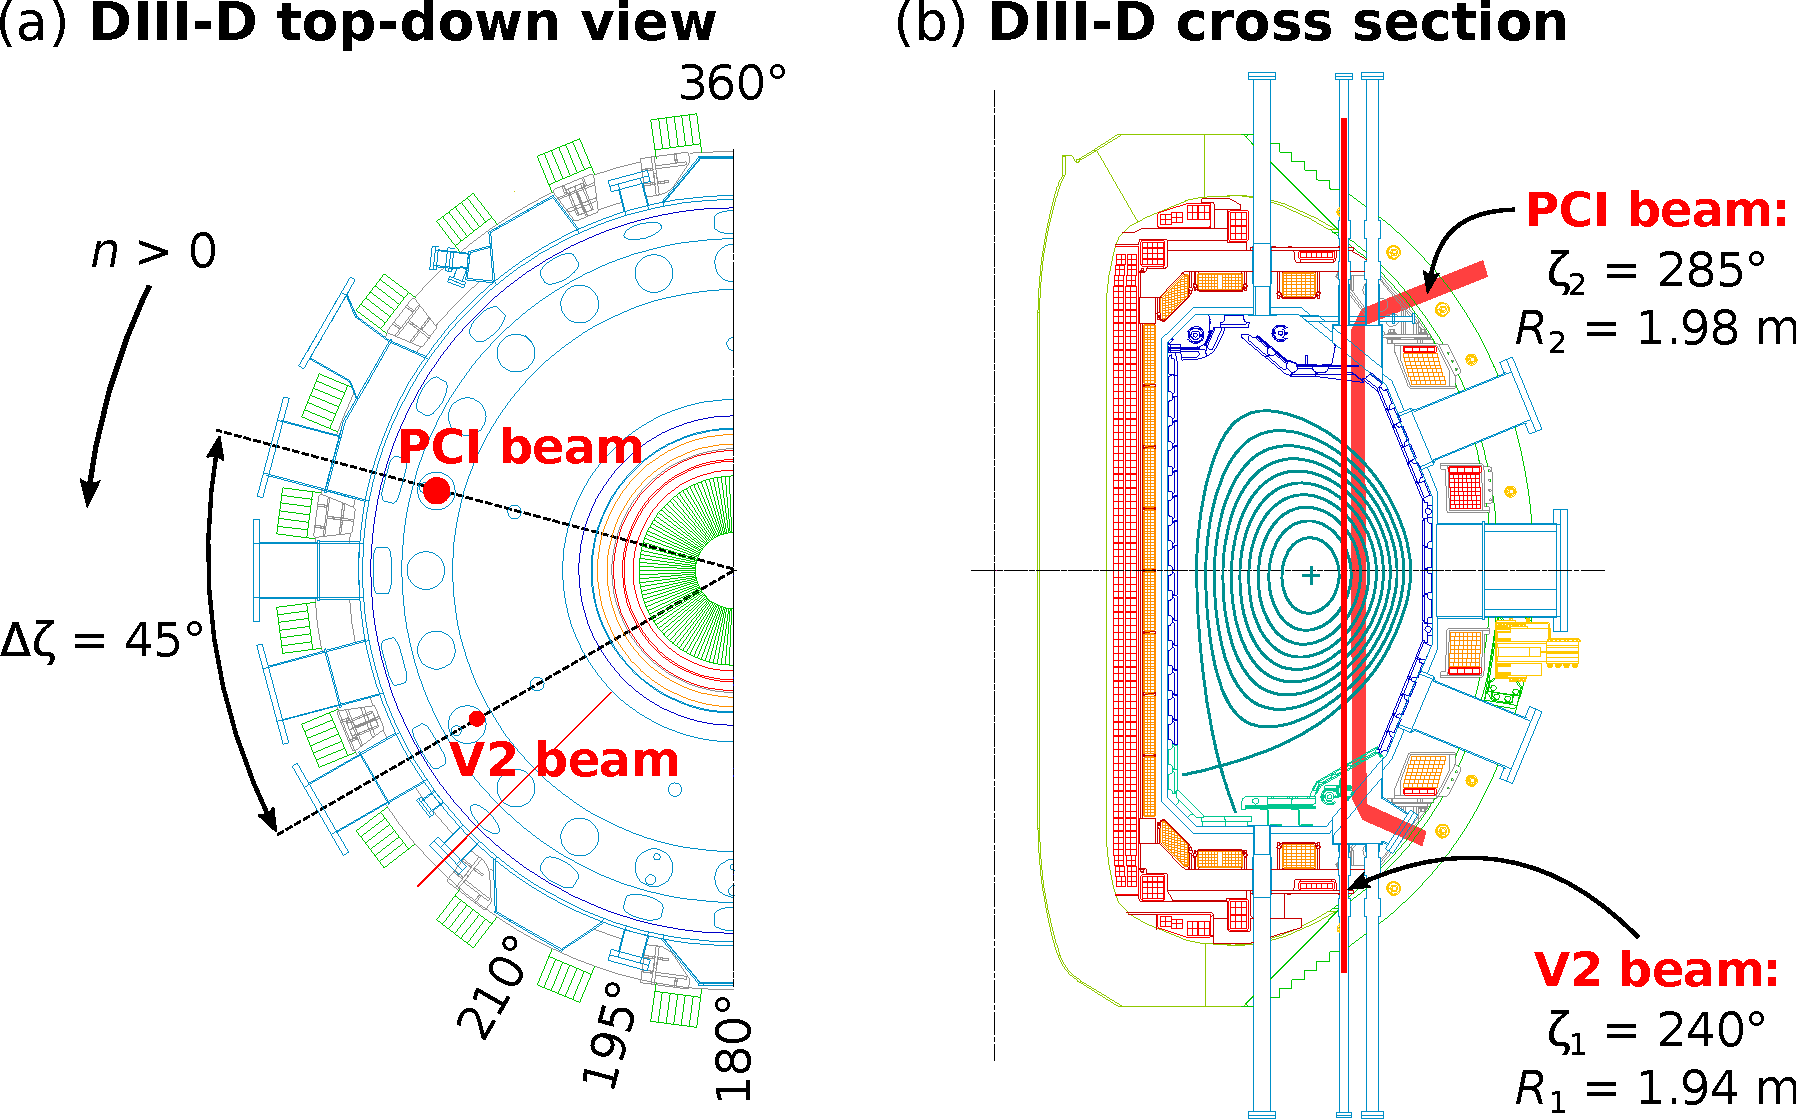
\includegraphics[width = \textwidth]{%
    Chapters/ToroidalCorrelation/figs/pci_interf_locs.pdf}
  \caption[Beam locations of the V2 and PCI interferometers on \diiid]{%
    (a) A top-down view of the \diiid\space vessel.
    The V2 interferometer beam's toroidal location is $\zeta_1 = 240^{\circ}$,
    and the PCI beam's toroidal location is $\zeta_2 = 285^{\circ}$.
    The \diiid\space sign convention for toroidal mode numbers
    is that $n > 0$ for modes that rotate counterclockwise
    when viewing the torus from above,
    as this corresponds to the direction of dominant torque injection.
    (b) A view of the \diiid\space cross section.
    The V2 interferometer beam's
    major-radial location is $R_1 = \SI{1.94}{\meter}$, and
    the PCI beam's major-radial location is $R_2 = \SI{1.98}{\meter}$.}
\label{fig:ToroidalCorrelation:pci_interf_locs}
\end{figure}

For completeness, it should also be mentioned that
a three-chord, radially viewing Faraday-effect polarimeter-interferometer
was recently installed on \diiid~\cite{chen_rsi16}.
While the primary impetus for this installation
is diagnosis of core-localized magnetic fluctuations,
it is also capable of making interferometric measurements
of line-integrated electron-density fluctuations.
The system sits at a toroidal location $285^{\circ}$ and
the radially viewing chords enter the vessel through the $R0$ port.
Presumably, these measurements could be correlated
with the $R0$ CO$_2$ heterodyne interferometer measurements
made at toroidal location $225^{\circ}$.
\graffito{\textcolor{red}{But are they really?}}
However, these two systems do not have phase-locked sampling rates
(the necessity of which is discussed in
Section~\ref{sec:ToroidalCorrelation:implementation_details_and_nonideal_effects:phase_locked_sampling}),
so no attempts to correlate these interferometric measurements
are made in this work.


\subsection{MHD plasma-density perturbations}
An MHD mode displaces a plasma from it's equilibrium position
by $\vect{\xi} = \vect{\xi}(\vect{r}, t)$.
The perturbed velocity is given as
$\vect{v}_1 = \partial \vect{\xi} / \partial t$
and, assuming harmonic variations, reduces to
\begin{equation}
  \vect{v}_1
  \equiv
  \frac{\partial \vect{\xi}}{\partial t}
  =
  -i \omega \vect{\xi},
  \notag
\end{equation}
where $\omega$ is the mode's angular frequency.
The plasma density $n_i$ is given as
\begin{equation}
  n_i = \bar{n}_i + \tilde{n}_i,
  \notag
\end{equation}
where $\bar{n}_i$ and $\tilde{n}_i$ are
the equilibrium and fluctuating components, respectively.
Assuming a stationary equilibrium ($\vect{v}_0 = 0$) and
using the above relations,
the linearized continuity equation reduces to
\begin{equation}
  \tilde{n}_i = -\nabla \cdot (\bar{n}_i \vect{\xi}).
  \label{eq:ToroidalCorrelation:density_fluctuations}
\end{equation}
If we relax the assumption on $\vect{v}_0$ to allow
finite equilibrium flow ($\vect{v}_0 \neq 0$),
then the right-hand side of (\ref{eq:ToroidalCorrelation:density_fluctuations})
is simply multiplied by the prefactor
$[1
- (\vect{v}_0 \cdot \vect{k} / \omega)
+ i (\nabla \cdot \vect{v}_0 / \omega)]^{-1}$, where
$\vect{k}$ is the mode wavevector.


\subsection{Interferometer-measured phase fluctuations}
The phase delay imparted to a CO$_2$ probe beam
propagating through a tokamak plasma
was discussed extensively in
Section~\ref{sec:InterferometricMethods:EM_waves_in_plasma}.
In particular, electron-density fluctuations $\tilde{n}_e$
produce phase fluctuations $\tilde{\phi}$ as given by
(\ref{eq:InterferometricMethods:phase_fluctuation}),
which is repeated here for completeness:
\graffito{\textcolor{red}{Sign???}}
\begin{equation}
  \tilde{\phi}
  =
  - r_e \lambda_0 \int \tilde{n}_e dl.
\end{equation}
Assuming quasineutrality $n_e \approx n_i$ and
invoking (\ref{eq:ToroidalCorrelation:density_fluctuations}),
these phase fluctuations reduce to
\begin{align}
  \tilde{\phi}
  =
  r_e \lambda_0
  \int [\nabla \cdot (\bar{n}_e \vect{\xi})] dl.
  \label{eq:ToroidalCorrelation:phase_fluctuations_from_displacement}
\end{align}

Now, \diiid's V2 and PCI interferometers have \emph{vertical} beam paths
located at major radial ($R$) and toroidal ($\zeta$) coordinates
$(R_1, \zeta_1) = (\SI{1.94}{\meter}, \; 240^{\circ})$ and
$(R_2, \zeta_2) = (\SI{1.98}{\meter}, \; 285^{\circ})$, respectively.
Fourier decomposing the displacement $\vect{\xi}$ as
\begin{equation}
  \vect{\xi}(\vect{r}, t)
  =
  \vect{\xi}_0(r) e^{i(m \theta + n \zeta - \omega t)}
  \notag
\end{equation}
for poloidal ($m$) and toroidal ($n$) mode numbers and
real $\vect{\xi_0}(r)$,
(\ref{eq:ToroidalCorrelation:phase_fluctuations_from_displacement}) becomes
\begin{align}
  \tilde{\phi}
  =
  r_e \lambda_0
  \int \left\{
    \nabla
    \cdot
    \left[
      \bar{n}_e \, \vect{\xi}_0(r) e^{i(m \theta + n \zeta - \omega t)}
    \right]
  \right\} dl.
  \notag
\end{align}
Finally, noting that $dl = dl(r, \theta)$ for vertical beam paths,
the phase fluctuations reduce to
\begin{equation}
  \tilde{\phi}
  =
  \Phi e^{i(n \zeta - \omega t)},
  \label{eq:ToroidalCorrelation:phase_fluctuations_vertical_beam1}
\end{equation}
where
$\Phi
\equiv
\Phi(R, m, n, \vect{\xi}_0(r), \bar{n}_e(r), \vect{G})$
is a complex-valued function of
the beam's major radial location,
the mode structure,
the equilibrium density profile, and
the plasma geometry $\vect{G} = \vect{G}(R_0, a, \kappa, \delta, \cdots)$.
$\Phi$ can be written explicitly
as a complex value $\Phi = |\Phi| e^{i \sigma}$.

For a given mode and plasma,
the V2 and PCI interferometer beams see the \emph{same}
$\{m, n, \vect{\xi}_0(r), \bar{n}_e(r), \vect{G}\}$, and
$\Phi$ reduces to a one-dimensional function $\Phi = \Phi(R)$.
Thus, (\ref{eq:ToroidalCorrelation:phase_fluctuations_vertical_beam1}) can
alternatively be written as
\begin{equation}
  \tilde{\phi}
  =
  |\Phi(R)| e^{i[n \zeta - \omega t + \sigma(R)]},
  \label{eq:ToroidalCorrelation:phase_fluctuations_vertical_beam2}
\end{equation}
where the dependence on $R$ for a given mode and plasma
has been noted explicitly.
The phase angle $\alpha$ of $\tilde{\phi}$ is defined as
\begin{equation}
  \alpha \equiv n \zeta - \omega t + \sigma(R)
  \label{eq:ToroidalCorrelation:phase_angle}
\end{equation}
such that $\tilde{\phi} = |\Phi| e^{i \alpha}$.


\subsection{The measured mode number --- the ideal case}
\graffito{\textcolor{red}{Do we have correct sign convention w/ $V2$}}
In the ideal case, phase fluctuations $\tilde{\phi}_1$ and $\tilde{\phi}_2$
are made at different toroidal locations $\zeta_1 \neq \zeta_2$ but
the \emph{same} radial locations $R_1 = R_2 = R$.
The one-sided cross-spectral density
$G_{12}(f) = |G_{12}(f)| e^{i \alpha_{12}(f)}$
then yields an estimate of the relative phase angle
$\alpha_{12} \equiv \alpha_2 - \alpha_1 = n(\zeta_2 - \zeta_1)$,
inspiring the definition of the measured toroidal mode number as
\begin{equation}
  n_{\text{meas}}
  \equiv
  \frac{\alpha_{12}}{\Delta \zeta},
  \quad \text{where} \quad
  \Delta \zeta \equiv \zeta_2 - \zeta_1.
  \label{eq:ToroidalCorrelation:toroidal_mode_number_ideal}
\end{equation}


\section{Implementation details and non-ideal effects}
\label{sec:ToroidalCorrelation:implementation_details_and_nonideal_effects}
Time-base discrepancies and offsets in major-radial position
between the $V2$ and PCI interferometers
can bias the measured mode number
(\ref{eq:ToroidalCorrelation:toroidal_mode_number_ideal})
away from the true toroidal mode number $n$.
As discussed below, time-base discrepancies have been eliminated
by phase locking the interferometers' sampling rates
(a hardware solution) and
by post-processing the digitized data
to remove the constant time-base offset
that results from the discrepancy
between each system's nominal and realized trigger times
(a software solution).
The major-radial offset of the interferometer probe beams
can result in tell-tale, artificial mode-number ``flips''.
Barring increased radial overlap (i.e.\ $\Delta R \rightarrow 0$),
interpretation of toroidal mode number measurements
from modes with substantial radial structure
\graffito{\textcolor{red}{forward-modeling ref}}
may require forward modeling.


\subsection{Phase-locked sampling}
\label{sec:ToroidalCorrelation:implementation_details_and_nonideal_effects:phase_locked_sampling}
Extracting useful information
from the correlation of two measurements
requires that the sampling rates of the two measurements
are \emph{phase-locked}.
If the sampling rates are \emph{not} phase-locked,
slippage between the sampling rates
will result in artificial evolution of the measured phase.

Digitizing the two signals on a common digitizer
is the simplest method for ensuring phase-locked sampling.
Unfortunately, such an approach is not suitable
for the $V2$ and PCI interferometer signals.
The $V2$ interferometer's
$f_{\text{IF}} = \SI{40}{\mega\hertz}$ intermediate-frequency signal
is demodulated using an all-digital technique
that mandates a use of a sampling rate
$f_s = (4 / 3) f_{\text{IF}}$
\cite{vanzeeland_rsi08}, and
the baseband $I$ and $Q$ signals never exist in analog form.
In contrast, as described in
Chapter~\ref{ch:Implementation} and \cite{davis_rsi16},
the PCI interferometer's
$f_{\text{IF}} = \SI{27}{\mega\hertz}$ intermediate-frequency signal
is demodulated with analog electronics, and
the analog baseband $I$ and $Q$ signals
are then digitized on two channels of a D-tAcq ACQ216 CPCI board.
Because the $V2$ interferometer's baseband $I$ and $Q$ signals
never exist in analog form,
it is not possible to digitize the $V2$ $I$ and $Q$ signals
on the digitizer used by the PCI interferometer.
Further, because of the intermediate-frequency mismatch
between the $V2$ and PCI interferometers,
it is also not possible digitally demodulate and digitize
the PCI interferometer's $\SI{27}{\mega\hertz}$ intermediate-frequency signal
using the $V2$ interferometer's
$\SI{40}{\mega\hertz}$ digital demodulation system.
An alternative approach is to directly digitize
both intermediate-frequency signals
with a high-bandwidth digitizer and
demodulate both signals in software,
as has been done elsewhere~\cite{mlynek_fst12}.
While \diiid's ion cyclotron emission (ICE) digitizer
has a $200 \, \text{MS/s}$ sample rate,
channels on the ICE digitizer are not consistently available.

As sharing a common digitizer is not possible,
phase-locked sampling between the $V2$ and PCI interferometers
requires that the digitizers of both systems
derive their clock from a common source.
The $V2$ interferometer derives its clock
from a free-running, oven-controlled oscillator
whose base frequency is $\SI{320}{\mega\hertz}$, and
the digital demodulation system
has two spare outputs that can be programmed
to output LVCMOS-level, phase-locked clock signals
at $\SI{320}{\mega\hertz} / N$, where
$N \in \{1, 2, 3, ..., 32\}$.
Both outputs are currently programmed with a divisor $N = 20$
such that they each provide a $\SI{16}{\mega\hertz}$ clock signal.
\graffito{\textcolor{red}{Picture? For posterity}}
One of these $\SI{16}{\mega\hertz}$ clock signals
is routed via coaxial cable
from the $V2$ digital demodulation hardware
in the first row of the \diiid\space ``annex''
to the PCI's digitizer
in the third row of the \diiid\space ``annex''.

The PCI digitizer typically samples at $f_s = 4 \, \text{MS/s}$.
Thus, division of the $V2$ $\SI{16}{\mega\hertz}$ clock by four
(in hardware or software) yields a clock appropriate for typical sampling.
Each board can accept an external clock
through the front panel's single-pin LEMO CLK input.
The CLK signal passes through an optocoupler
with a bandwidth $\sim \SI{10}{\mega\hertz}$
\cite{milne_optocoupler_pc16}, but
in-house tests have demonstrated
that the input clock frequency
can actually exceed $\SI{16}{\mega\hertz}$.
As a result, the $\SI{16}{\mega\hertz}$ signal
is directly connected to the front panel CLK lemo input, and
the necessary division
(e.g.\ divide by four to achieve typical $4 \, \text{MS/s}$ sampling rate)
is performed within the digitizer;
it is the author's opinion that
this is cleaner, simpler, and more easily extensible
(i.e.\ easier to implement other sampling rates)
than performing the division in hardware.
Details of the signal routing and the clock division
are provided in Appendix~\ref{app:ExternalClock}.
Thus, as of June 2016,
the $V2$ and PCI interferometer sampling rates
are phase-locked.


\subsection{Eliminating the time-base offset}
The V2 and PCI interferometer sampling rates are phase-locked,
as both systems share a common clock.
However, phase-locked sampling rates do \emph{not} guarantee
identical/ideal \emph{triggering} of both systems, so
there could very well be an offset between the
V2 and PCI interferometer time bases.

Imagine that the time bases between $\tilde{\phi}_1$ and $\tilde{\phi}_2$
are offset by constant $\delta t$ such that
$t_1 \equiv t$ and $t_2 \equiv t + \delta t$.
Then, for \emph{constant} angular frequency ($\omega = \text{const}$),
$\alpha_{12} = n \Delta \zeta - \omega \delta t$
such that application of
(\ref{eq:ToroidalCorrelation:toroidal_mode_number_ideal})
yields a measured mode number
\begin{equation}
  n_{\text{meas}} = n - \frac{\omega \delta t}{\Delta \zeta}.
  \label{eq:ToroidalCorrelation:toroidal_mode_number_dt_constant_omega}
\end{equation}
That is, the measured mode number will be biased away from
the true mode number by a constant DC offset.
If the true mode number $n$ is known,
then (\ref{eq:ToroidalCorrelation:toroidal_mode_number_dt_constant_omega})
can be used to determine the time-base offset $\delta t$.

Now, in addition to constant time offset $\delta t$,
imagine that the mode's angular frequency is ramping linearly in time
($\dot{\omega} = \partial \omega / \partial t = \text{const}$) such that
$\omega(t + \delta t) = \omega(t) + \dot{\omega} \delta t$.
Then,
$\alpha_{12}
=
n \Delta \zeta - [\omega(t)] \delta t - (\dot{\omega} \delta t) t$
such that application of
(\ref{eq:ToroidalCorrelation:toroidal_mode_number_ideal})
yields a measured mode number that also ramps linearly in time
\begin{equation}
  \dot{n}_{\text{meas}}
  =
  - \left( \frac{2 \dot{\omega}}{\Delta \zeta} \right) \delta t.
  \label{eq:ToroidalCorrelation:toroidal_mode_number_dt_ramp_rate}
\end{equation}
Note that (\ref{eq:ToroidalCorrelation:toroidal_mode_number_dt_ramp_rate}) is
\emph{independent} of the true toroidal mode number $n$,
unlike (\ref{eq:ToroidalCorrelation:toroidal_mode_number_dt_constant_omega}).
Further, if $\delta t$ is ``large''
(i.e.\ $|\omega \delta t / \Delta \zeta| > n_{\text{Ny}}$),
$n_{\text{meas}}$ may be aliased and application of
(\ref{eq:ToroidalCorrelation:toroidal_mode_number_dt_constant_omega})
will give an incorrect value for $\delta t$.
Thus, if the frequency of the mode is ramping \emph{and}
the measured toroidal mode number $n_{\text{meas}}$ is also ramping in time,
(\ref{eq:ToroidalCorrelation:toroidal_mode_number_dt_ramp_rate})
can be used to determine the time-base offset $\delta t$ and
is superior to application of
(\ref{eq:ToroidalCorrelation:toroidal_mode_number_dt_constant_omega}).

\graffito{\textcolor{red}{Improve explanation}}
To make use of (\ref{eq:ToroidalCorrelation:toroidal_mode_number_dt_ramp_rate}),
$\dot{\omega}$ must be computed from experimental measurements.
Note that the \emph{measured} angular frequency is given as
$\omega_{\text{meas}} \equiv \partial[\omega(t) \cdot t] / \partial t$.
In the case where $\omega = \text{const}$,
this yields the expected result that $\omega_{\text{meas}} = \omega$.
However, if the angular frequency is ramping linearly in time
($\omega(t) = \omega_0 + \dot{\omega} t$), then
$\omega_{\text{meas}} = \omega_0 + 2 \dot{\omega} t$ and
$\dot{\omega}_{\text{meas}} = 2 \dot{\omega}$.
Thus, (\ref{eq:ToroidalCorrelation:toroidal_mode_number_dt_ramp_rate}) becomes
\begin{equation}
  \dot{n}_{\text{meas}}
  =
  - \left( \frac{\dot{\omega}_{\text{meas}}}{\Delta \zeta} \right) \delta t.
  \label{eq:ToroidalCorrelation:toroidal_mode_number_dt_ramp_rate_lab_frame}
\end{equation}

\begin{figure}
  \centering
  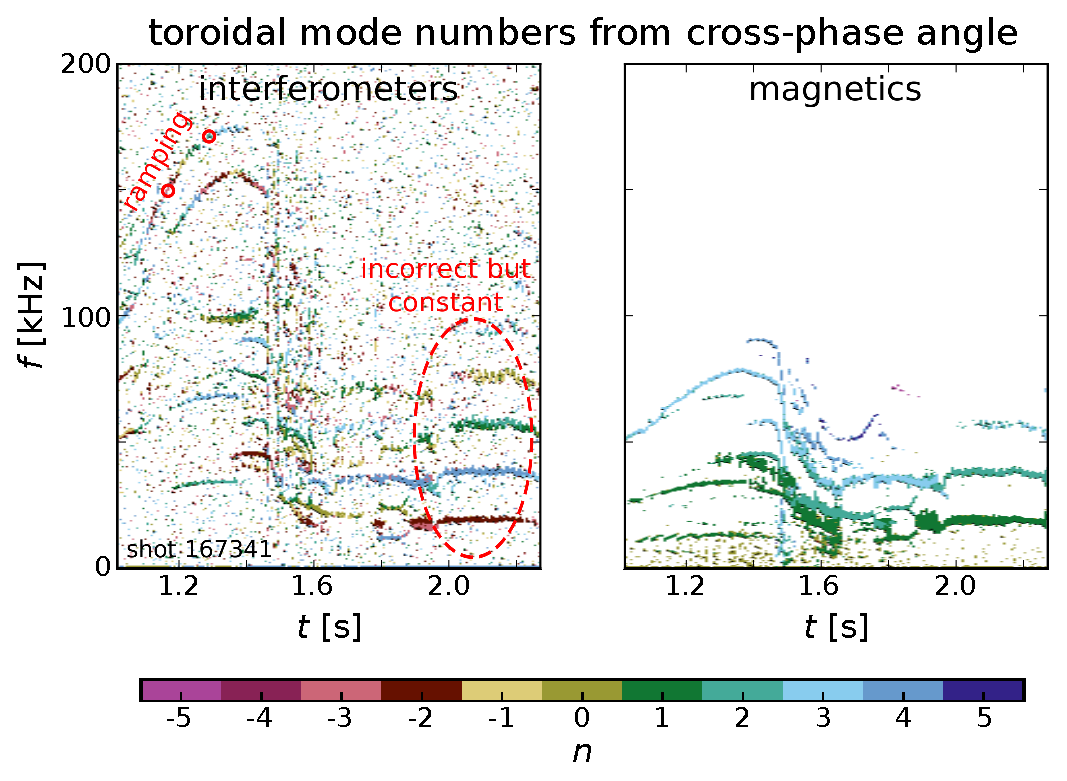
\includegraphics[width = \textwidth]{%
    Chapters/ToroidalCorrelation/figs/mode_numbers_with_uncompensated_time_delay.eps}
  \caption[Effect of uncompensated time delay on computed toroidal mode numbers]{%
    Computed mode numbers from
    toroidally separated interferometers and magnetics.
    When there is an uncompensated time delay ($\delta t \neq 0$)
    between the two interferometers, as there is here,
    the interferometer-measured mode numbers
    for both constant-frequency and ramping-frequency modes
    are \emph{incorrectly} computed.}
\label{fig:ToroidalCorrelation:uncompensated_time_delay}
\end{figure}

\graffito{\textcolor{red}{Improve discussion of two estimates}}
Now, Fig.~\ref{fig:ToroidalCorrelation:uncompensated_time_delay} shows an example
of the computed toroidal mode number spectrum
when using the native time-bases of the V2 and PCI interferometers;
the corresponding magnetics spectrum is shown for comparison.
For $t \lesssim \SI{1.5}{\second}$
the mode frequencies are ramping approximately linearly in time, and
the interferometer-measured mode number is (artificially) ramping in time,
in contrast to the corresponding measurements from magnetics;
application of
(\ref{eq:ToroidalCorrelation:toroidal_mode_number_dt_ramp_rate_lab_frame})
to the \emph{highest-frequency} mode observed by the interferometers yields
$\delta t \approx \SI{-30}{\micro\second}$
($\Delta n = 5$, $\Delta f \approx \SI{20}{\kilo\hertz}$,
as indicated by the positions of the small circular annotations
to the highest frequency mode in
Fig.~\ref{fig:ToroidalCorrelation:uncompensated_time_delay}).
Further, note that the mode number evolution \emph{reverses}
after the mode reaches its peak frequency,
in agreement with the behavior expected from
(\ref{eq:ToroidalCorrelation:toroidal_mode_number_dt_ramp_rate_lab_frame}).
Finally, for $t \gtrsim \SI{2}{\second}$
the mode frequencies are constant, but
the interferometer-measured mode numbers are in disagreement with magnetics.
Naive application of
(\ref{eq:ToroidalCorrelation:toroidal_mode_number_dt_constant_omega})
to the \emph{lowest-frequency} mode at $f \approx \SI{20}{\kilo\hertz}$
yields $\delta t \approx \SI{20}{\micro\second}$
($n_{\text{meas}} = -2$, $n = 1$,
$\omega \approx 2 \pi \cdot \SI{20}{\kilo\hertz}$),
in contrast with the above time-delay estimate
from the linearly ramping mode numbers.
However, as warned above,
$n_{\text{meas}}$ will be \emph{aliased} for ``large'' time delays:
using the above parameters for the lowest-frequency mode,
we see that $|\omega \delta t / \Delta \zeta| \approx 4.8 > n_{\text{Ny}}$,
where $n_{\text{Ny}} = 4$ is the Nyquist mode number
for the $\Delta \zeta = 45^{\circ}$ toroidal separation of the interferometers,
confirming that aliasing has biased the time-delay estimate.
To account for aliasing, take $n_{\text{meas}} = -2 \rightarrow 6$, and
application of
(\ref{eq:ToroidalCorrelation:toroidal_mode_number_dt_constant_omega}) yields
$\delta t \approx -\SI{30}{\micro\second}$,
in agreement with the time-delay estimate
from the linearly ramping mode numbers!

The above observations are all consistent with there being an offset
between the native time-bases of the PCI and V2 interferometers, and
the two \emph{independent} measurements of this time offset are in agreement,
with each yielding an offset $\delta t \approx \SI{-30}{\micro\second}$.
Indeed, delaying the PCI signal by $-\SI{30}{\micro\second}$
relative to the V2 signal in software dramatically improves
the agreement between the interferometer and magnetics mode number spectra.
By scanning $\delta t$ about $-\SI{30}{\micro\second}$ and
noting when discrepancy with magnetics began to creep back into
the interferometer-measured mode spectrum,
the upper and lower bounds of $\delta t$ were found;
the best estimate for $\delta t$ was then taken as the midpoint
between these upper and lower bounds, which was found to be
\begin{equation}
  \delta t = -\SI{32}{\micro\second}.
  \label{eq:ToroidalCorrelation:time_delay}
\end{equation}
That is, the native PCI-interferometer's time base \emph{leads}
the native V2 time base by $\SI{32}{\micro\second}$.
Delaying the PCI-interferometer by $\SI{32}{\micro\second}$ (in software)
relative to the V2 interferometer yields the mode number spectrum
shown in Fig.~\ref{fig:ToroidalCorrelation:compensated_time_delay}.
Note that both
Fig.~\ref{fig:ToroidalCorrelation:uncompensated_time_delay} and
Fig.~\ref{fig:ToroidalCorrelation:compensated_time_delay}
correspond to shot 167341, and
the only difference in the interferometer-measured mode-number spectrum
between the two figures results from the compensation of the time delay
between the native time bases of the two interferometers.

\textcolor{red}{Note that additional measurements are needed
to determine which clock is correct in the \emph{absolute} sense.
For example, we can try digitizing a trigger signal and
comparing the digitized time of the trigger to the ``nominal'' trigger time
to determine the offset of our digitizer from the DIII-D clock.}

\begin{figure}
  \centering
  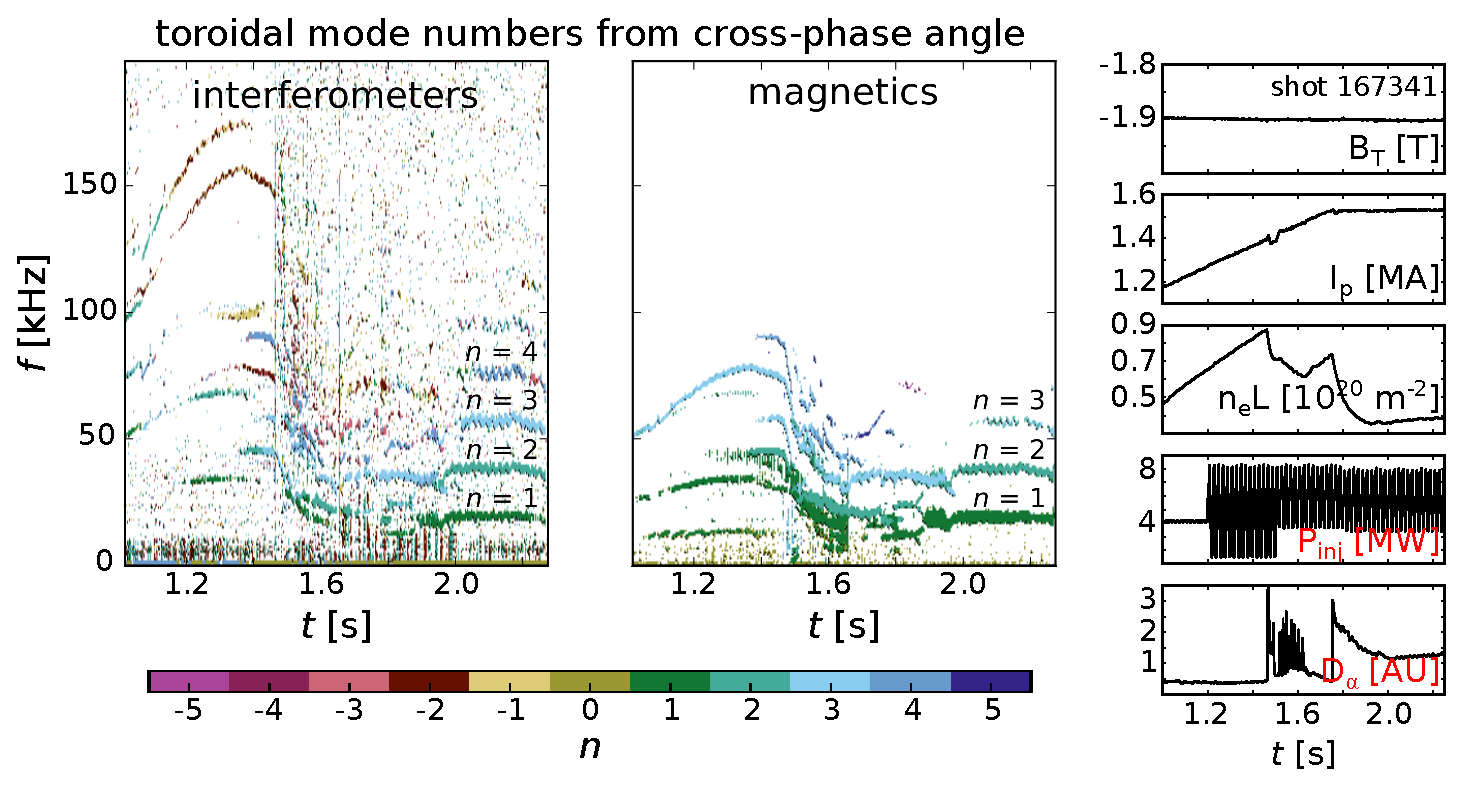
\includegraphics[width = \textwidth]{%
    Chapters/ToroidalCorrelation/figs/magnetics_and_interferometer_mode_numbers_167341.eps}
  \caption[Computed toroidal mode numbers \emph{after} removing time delay
      from Fig.~\ref{fig:ToroidalCorrelation:uncompensated_time_delay}]{%
    Computed mode numbers from
    toroidally separated interferometers and magnetics.
    Here, the PCI-interferometer signal has been delayed by
    $\SI{32}{\micro\second}$ relative to the V2 signal
    to account for the time offset between each system's native time base.
    Note that the agreement with magnetics is excellent and that
    the mode numbers of the ramping-frequency modes are no longer
    artificially ramping;
    this is an enormous improvement over the corresponding
    uncompensated interferometer-measured spectrum in
    Fig.~\ref{fig:ToroidalCorrelation:uncompensated_time_delay}.}
\label{fig:ToroidalCorrelation:compensated_time_delay}
\end{figure}


\subsection{Effects of radial offset}
\label{sec:ToroidalCorrelation:implementation_details_and_nonideal_effects:radial_offset}
\begin{itemize}
  \item \textcolor{red}{ECE to confirm radial mode structure}
  \item \textcolor{red}{Correlate $V1$, $V2$, $V3$ to see just radial effect}
\end{itemize}
The V2 and PCI interferometer beam paths have a slight radial offset
($\Delta R = \SI{4}{\centi\meter}$ with
$R_{\text{V2}} = \SI{1.94}{\meter}$ and $R_{\text{PCI}} = \SI{1.98}{\meter}$).
Thus, $\alpha_{12} = n(\zeta_2 - \zeta_1) + [\sigma(R_2) - \sigma(R_1)]$,
where
\begin{equation}
  \sigma(R_2) - \sigma(R_1)
  \approx
  \begin{cases}
    0, & \quad \text{$\vect{\xi}(R_1)$ and $\vect{\xi}(R_2)$ in-phase} \\
    \pi, & \quad \text{$\vect{\xi}(R_1)$ and $\vect{\xi}(R_2)$ out-of-phase}
  \end{cases},
  \notag
\end{equation}
gives the relative phase of $\vect{\xi}$
at $R_2$ relative to that at $R_1$.
If $\vect{\xi}(R_1)$ and $\vect{\xi}(R_2)$ are in-phase,
then application of (\ref{eq:ToroidalCorrelation:toroidal_mode_number_ideal})
will yield the correct mode number.
However, if $\vect{\xi}(R_1)$ and $\vect{\xi}(R_2)$ are out-of-phase,
then application of (\ref{eq:ToroidalCorrelation:toroidal_mode_number_ideal})
will yield a measured mode number $n_{\text{meas}}$
\graffito{\textcolor{red}{Correct sign for alias??}}
\begin{equation}
  n_{\text{meas}}
  =
  \begin{cases}
    n + n_{\text{Ny}}, & \quad n \leq 0 \\
    n - n_{\text{Ny}}, & \quad n > 0
  \end{cases},
  \label{eq:ToroidalCorrelation:toroidal_mode_number_radially_out_of_phase}
\end{equation}
where $n_{\text{Ny}} \equiv \pi / \Delta \zeta$
is the Nyquist toroidal mode number, and
the $n > 0$ case results from \emph{aliasing}
(that is, $n + n_{\text{Ny}} \rightarrow n - n_{\text{Ny}}$
when $n > 0$ because of aliasing).
Lacking additional measurements or some type of forward modeling,
this incorrect mode-number identification may go undiagnosed.
However, if $\vect{\xi}(R)$ evolves such that
$\vect{\xi}(R_1)$ and $\vect{\xi}(R_2)$ transition
from being in-phase to being out-of-phase (or vice versa),
the measured mode number will ``flip'';
an example of this mode-number ``flipping''
is shown in Fig.~\ref{fig:ToroidalCorrelation:mode_number_flips}.
Further effects of the radial offset can be investigated
via forward modeling.

\begin{figure}
  \centering
  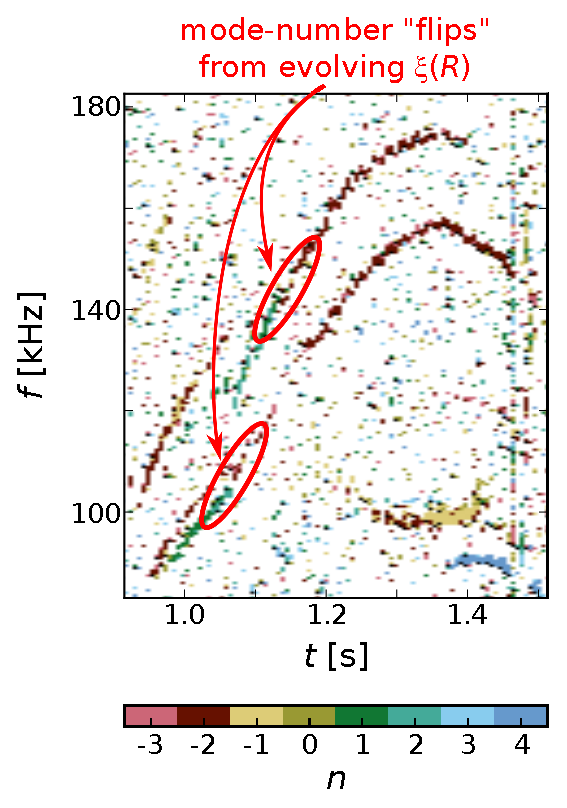
\includegraphics[width = 0.5 \textwidth]{%
    Chapters/ToroidalCorrelation/figs/phase_flips_167341.eps}
  \caption[Mode-number ``flipping'' due to the small radial offset
      between the $V2$ and PCI interferometers]{%
    Due to the small radial offset ($\Delta R = \SI{4}{\centi\meter}$)
    between the V2 and PCI interferometers,
    changes in the radial structure of a mode
    can result in ``flipping'' of the interferometer-measured mode number.
    Here, the mode number flips from $n = 2$ to $n = -2$,
    consistent with
    (\ref{eq:ToroidalCorrelation:toroidal_mode_number_radially_out_of_phase}).
    Lacking additional measurements or some type of forward modeling,
    it is impossible to determine if the mode is truly $n = 2$ or $n = -2$.
    Note that these modes exceed the typical bandwidth of magnetics, however,
    so even identification as $n = \pm 2$ \emph{is} an improvement!}
\label{fig:ToroidalCorrelation:mode_number_flips}
\end{figure}


\section{Example mode number spectra}
\label{sec:ToroidalCorrelation:survey_of_spectra}
\textcolor{red}{%
  This section contains representative results
  from the toroidal correlation measurement
  obtained over the very brief ``metal-rings'' campaign (June 2016).
  This is \emph{not} a complete section,
  as it consists solely of figures and detailed captions.
  This is intended to be a survey of current measurements.
  In the final version of my thesis,
  some of these figures (or variants thereof)
  may be moved to other chapters, and
  I may decide to only keep a few of the figures
  in this section for detailed discussion.
  Obviously, your insight will be helpful
  for pruning and focusing this section.
}

\begin{figure}[h!]
  \centering
  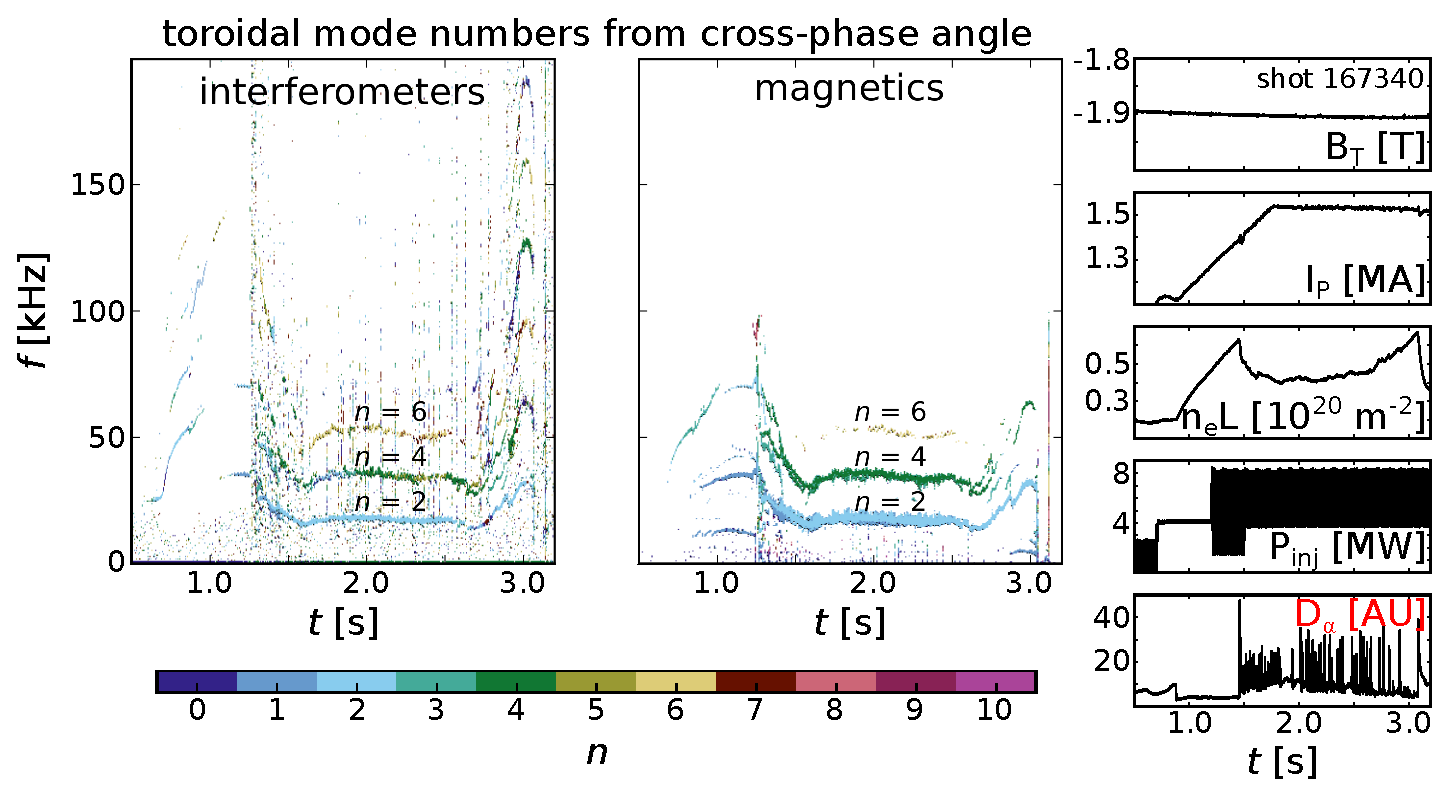
\includegraphics[width = \textwidth]{%
    Chapters/ToroidalCorrelation/figs/magnetics_and_interferometer_mode_numbers_167340.eps}
  \caption[Another example of excellent agreement between the
      interferometer and magnetics mode number spectra]{%
    Another example of excellent agreement between the
    interferometer and magnetics mode number spectra. Note that
    the interferometers additionally see modes \emph{invisible} to magnetics.
    Here,the modes were \emph{assumed} to be rotating
    in the ``positive'' direction
    (i.e.\ counterclockwise when viewing the torus from above,
    as this corresponds to the direction of dominant torque injection)
    such that we can discriminate $0 \leq n < 8$
    (rather than the typical $-4 < n \leq 4$).}
\label{fig:ToroidalCorrelation:magnetics_corroboration_2}
\end{figure}

\begin{figure}[h!]
  \centering
  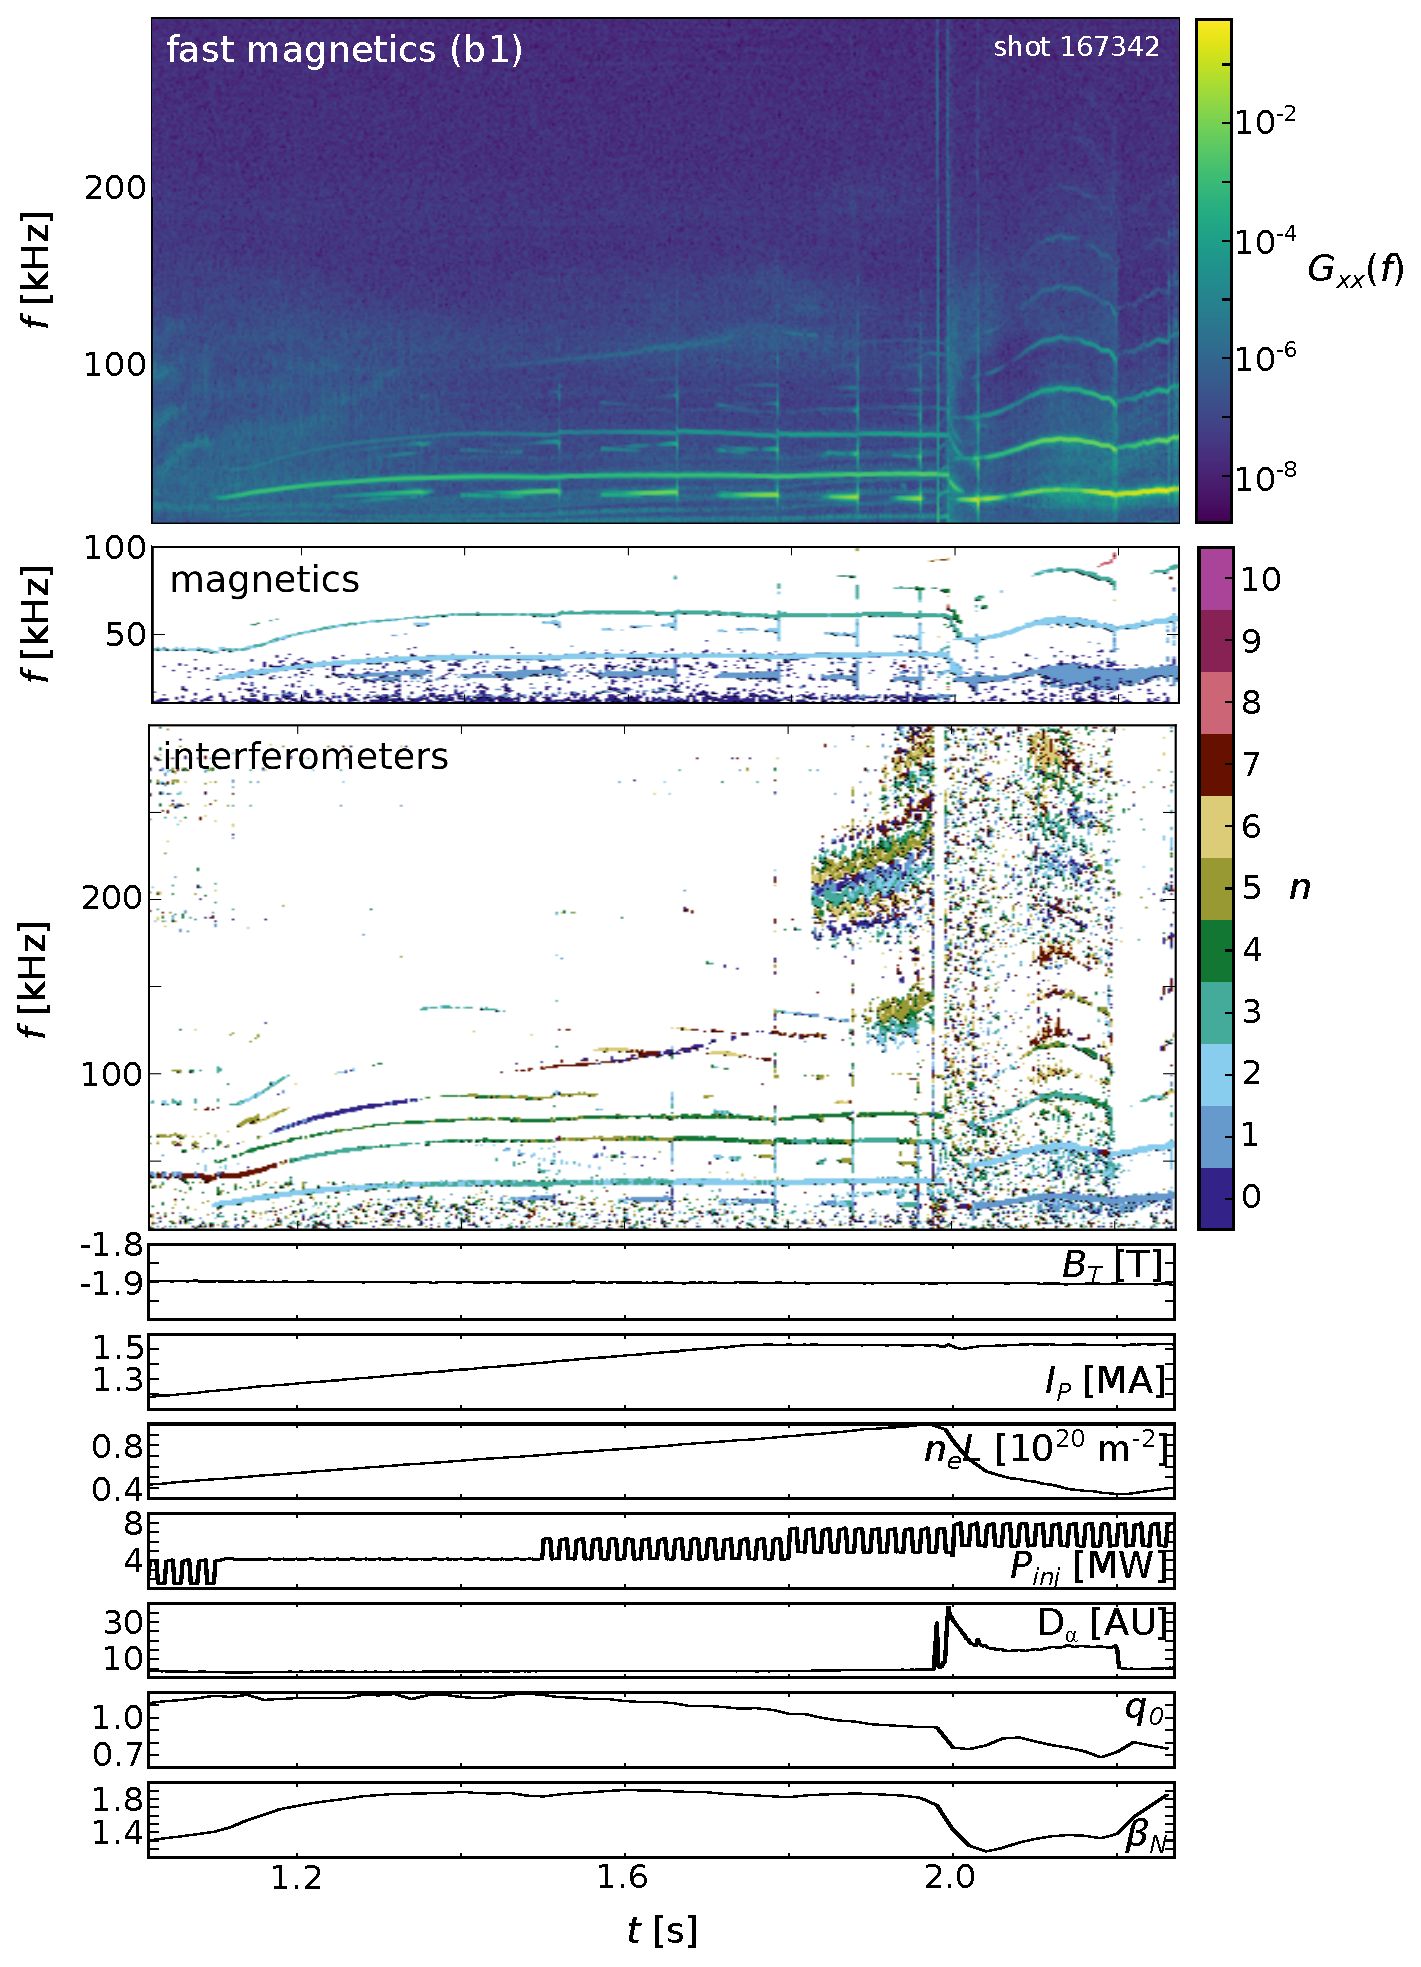
\includegraphics[width = 0.8 \textwidth]{%
    Chapters/ToroidalCorrelation/figs/core_localized_167342.eps}
  \caption[Toroidal mode numbers of \emph{core-localized} MHD]{%
    Between $1.8 \leq t \, [\text{s}] \leq 2.2$,
    the correlated interferometers measure fluctuations
    (Alfv\'{e}n eigenmodes?) that are \emph{invisible} to magnetics.
    This suggests that the modes are \emph{core-localized} and
    that the correlated interferometers are indeed capable
    of measuring core-localized MHD!
    (Note that the fast magnetic probes have a \SI{1}{\mega\hertz} bandwidth,
    but they do not have significant toroidal separation,
    preventing accurate measurement of toroidal mode numbers).}
\label{fig:ToroidalCorrelation:core_localized}
\end{figure}

\begin{figure}[h!]
  \centering
  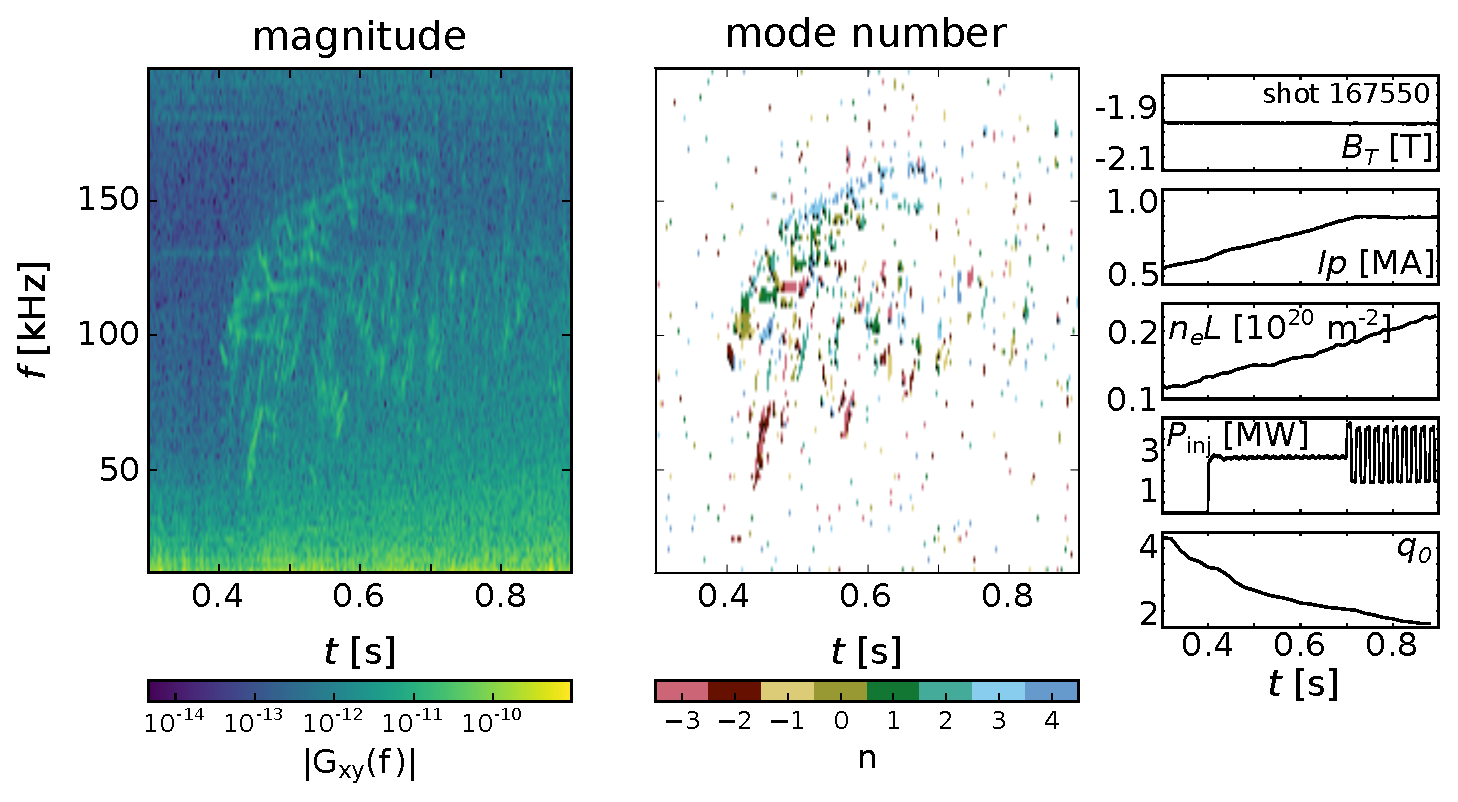
\includegraphics[width = \textwidth]{%
    Chapters/ToroidalCorrelation/figs/AEs_167550.eps}
  \caption[Toroidal mode numbers of Alfv\'{e}n eigenmodes]{%
    Alfv\'{e}n eigenmodes visible
    on the correlated interferometers.
    These modes are not readily visible on magnetics.}
\label{fig:ToroidalCorrelation:AEs}
\end{figure}

\begin{figure}[h!]
  \centering
  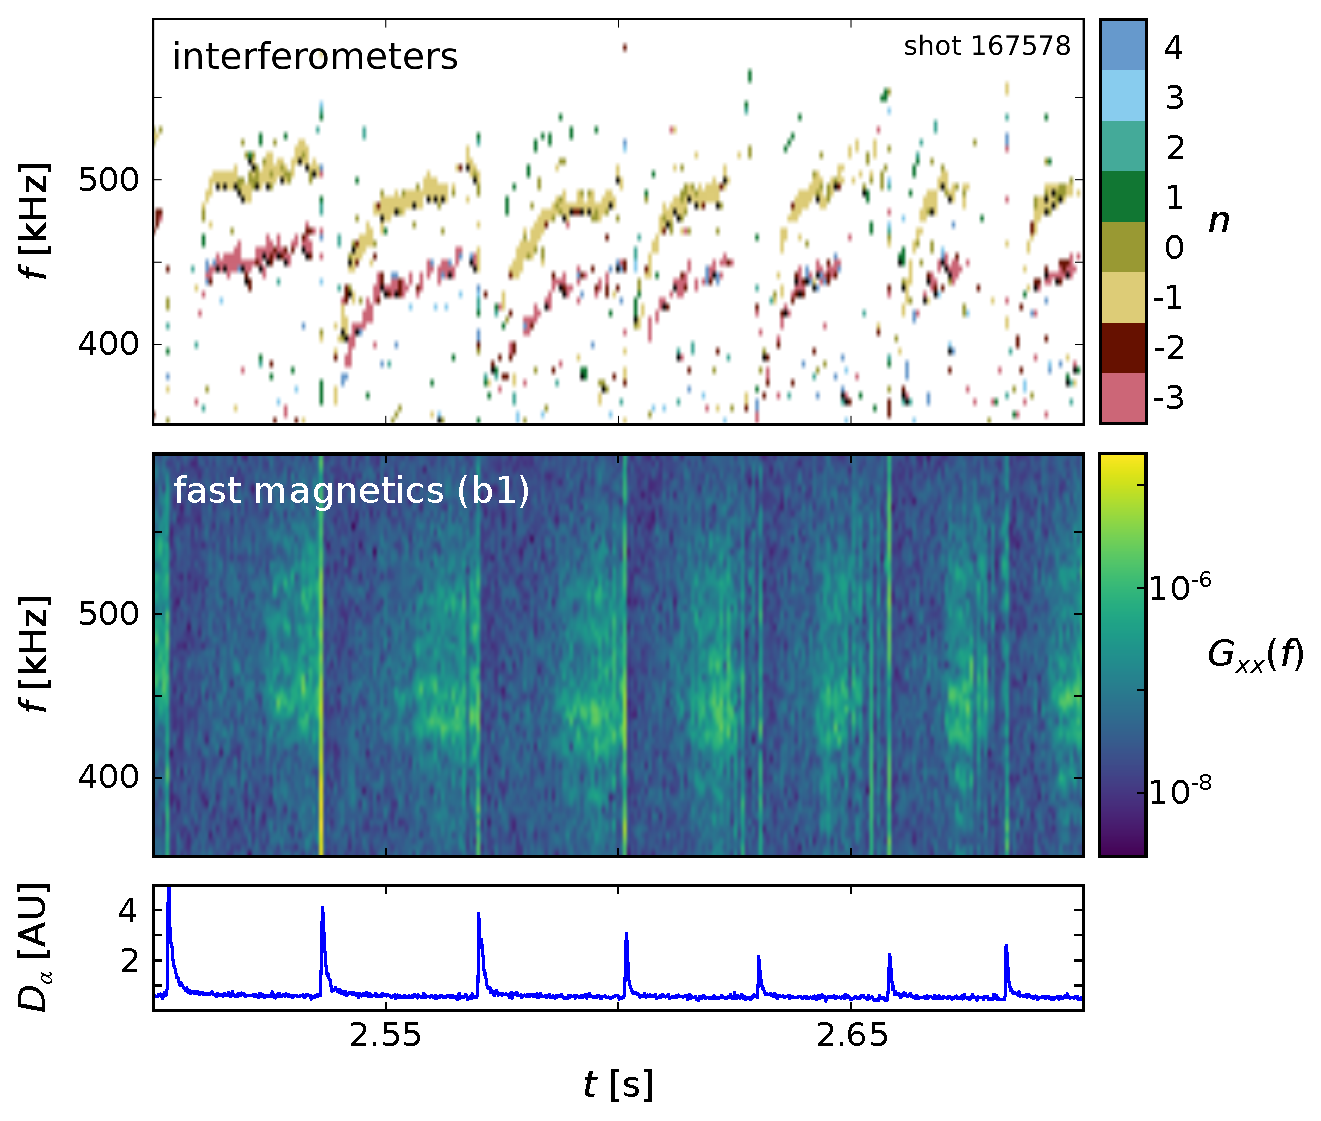
\includegraphics[width = 0.7 \textwidth]{%
    Chapters/ToroidalCorrelation/figs/interELM_fast_167578.eps}
  \caption[Toroidal mode numbers of inter-ELM fluctuations]{%
    Inter-ELM fluctuations as measured by
    the correlated interferometers and fast magnetics.
    The mode frequency ramps early in the inter-ELM window before saturating;
    the magnetic component of the fluctuation only appears \emph{after}
    the mode frequency has saturated --- fascinating!
    (Note that the fast magnetic probes have a \SI{1}{\mega\hertz} bandwidth,
    but they do not have significant toroidal separation,
    preventing accurate measurement of toroidal mode numbers).
    The drive and significance of such fluctuations is not known, but
    they do \emph{not} occur in every ELMy discharge.}
\label{fig:ToroidalCorrelation:interELM_fast}
\end{figure}

\begin{figure}[h!]
  \centering
  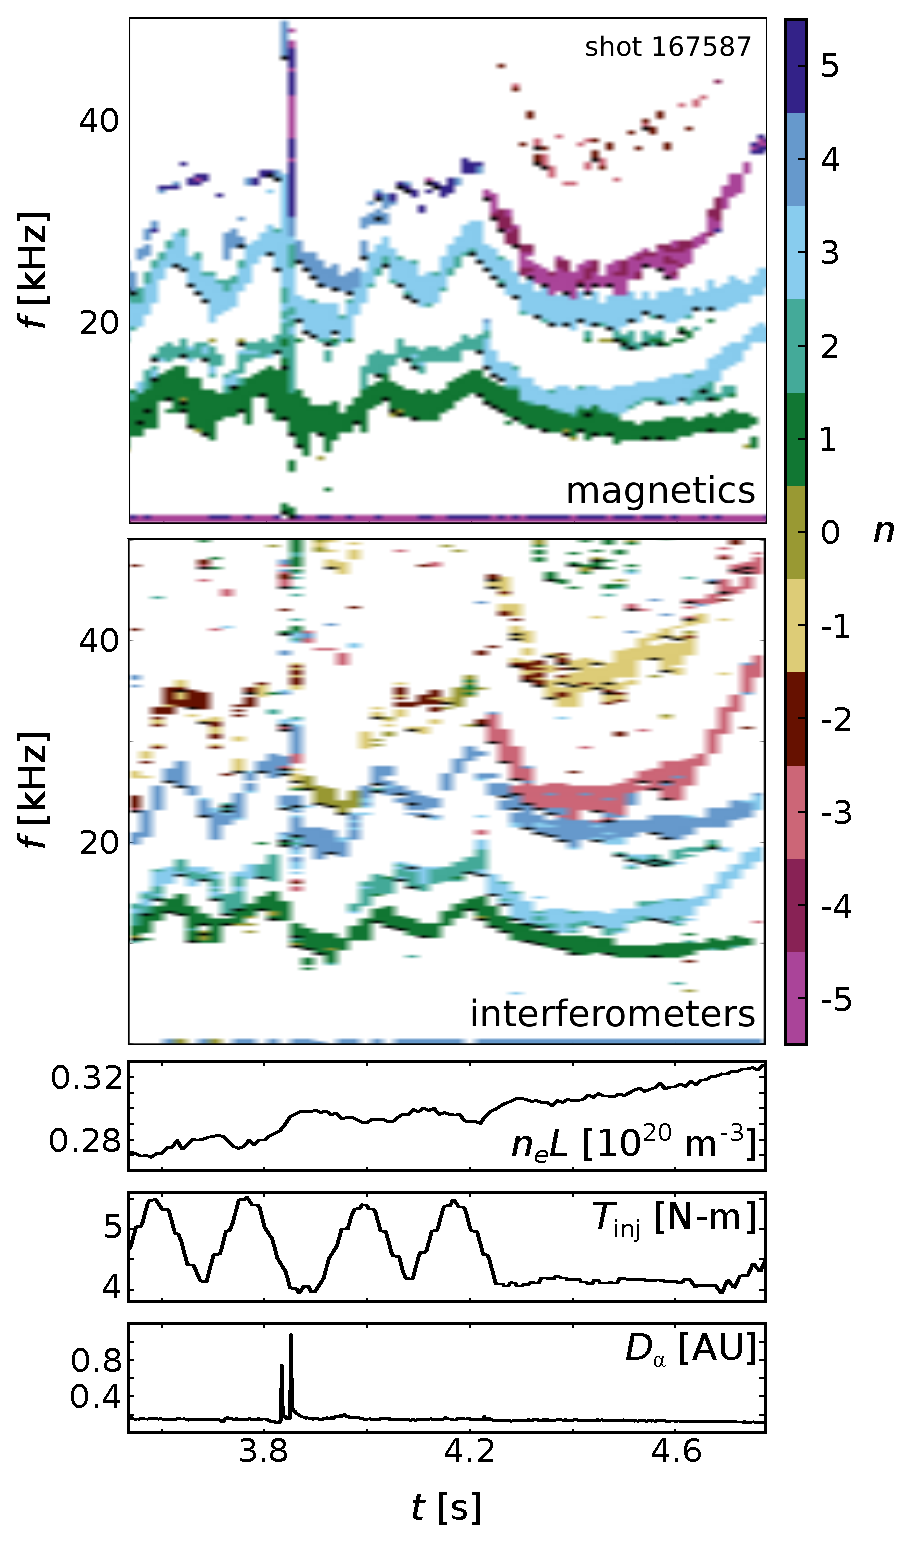
\includegraphics[width = 0.5 \textwidth]{%
    Chapters/ToroidalCorrelation/figs/EHO_167587.eps}
  \caption[Toroidal mode numbers of the edge harmonic oscillation (EHO)]{%
    The magnetics and interferometers both see the
    edge harmonic oscillation (EHO), which is responsible for
    flushing impurities from quiescent H-mode (QH-mode) plasmas.
    Below \SI{20}{\kilo\hertz}, the magnetics and interferometers
    both measure the same toroidal mode numbers; however,
    above \SI{20}{\kilo\hertz}, the measured mode numbers differ,
    likely due to a combination of aliasing and the small radial offset
    of the two interferometer beams.}
\label{fig:ToroidalCorrelation:EHO}
\end{figure}

\begin{figure}[h!]
  \centering
  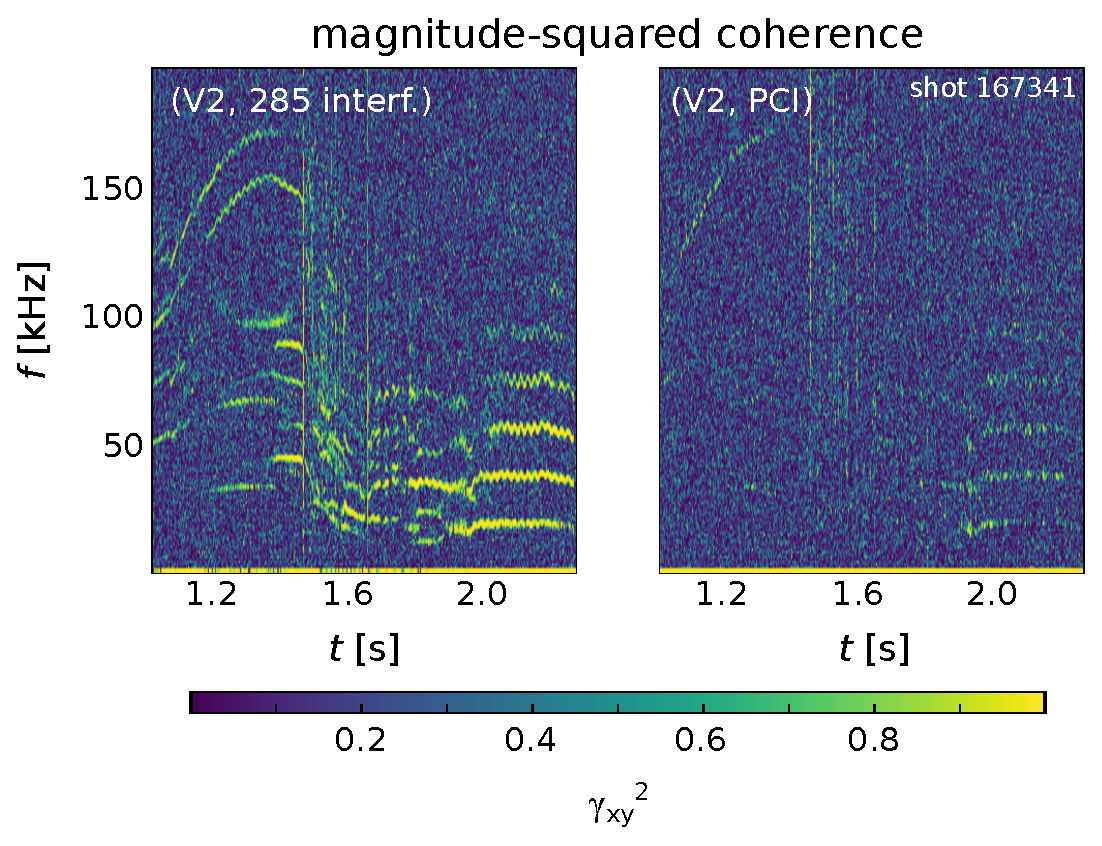
\includegraphics[width = 0.75 \textwidth]{%
    Chapters/ToroidalCorrelation/figs/interferometer_vs_PCI_coherence.eps}
  \caption[Inability to correlate V2 and PCI]{%
    The magnitude-squared coherence $\gamma_{xy}^2$ between
    the V2 and 285 interferometers (left) and
    between the V2 interferometer and PCI (right).
    The high coherence between the V2 and 285 interferometers
    allows accurate measurement of toroidal mode numbers,
    as demonstrated by the corresponding mode number spectrum
    displayed in Fig.~\ref{fig:ToroidalCorrelation:compensated_time_delay},
    whereas the poor coherence between the V2 and PCI
    prevents such measurements.
    (Note that ``285 interferometer'' refers to
    the newly installed interferometer channel of the PCI).}
\label{fig:ToroidalCorrelation:PCI_coherence}
\end{figure}


\bibliographystyle{plainurl}
\bibliography{references}
